\documentclass[autodetect-engine,dvipdfmx-if-dvi,ja=standard,a4j,jbase=11pt,magstyle=nomag*]{bxjsreport}
% \documentclass[uplatex, dvipdfmx, a4paper, 11ptj, report]{jsbook}
% small japanese font size:     9pt, 10pt, 11pt, 12pt, 14pt, ... (please refer the document of jsclasses)
% word-like japanese font size: 10ptj 10.5ptj, 11ptj, 12ptj (or jbase=xxpt (without 'j') if error is occured)
    
\usepackage{ifptex,ifxetex,ifluatex}
\ifluatex
    \usepackage{bxcalcux}
    \ltjsetparameter{jacharrange={-2,-3}}
    \usepackage{luatexja-otf}
    \usepackage{bxbase}
\else\ifxetex
    % \usepackage{zxjatype}
    % \usepackage[macros]{zxotf}
    \XeTeXgenerateactualtext=1
    \usepackage{xltxtra}
    \usepackage{bxbase}
\else\ifuptex
    \usepackage{otf}
    \usepackage[prefernoncjk]{pxcjkcat}
    \cjkcategory{sym11,sym18,sym19}{cjk}
    \usepackage[utf8]{inputenc}
    \usepackage{pxbase}
\else\ifstrictptex
    \usepackage{otf}
    \usepackage[utf8]{inputenc}
    \usepackage{pxbase}
\fi\fi\fi\fi

\usepackage[LGR,T2A,T1]{fontenc}

\usepackage{graphicx}
% \usepackage[dvipdfmx]{graphicx}
\usepackage{grffile}

% paper layout setting
\setpagelayout{noheadfoot, left=18.0truemm, right=18.0truemm, top=29.0truemm, bottom=26.0truemm, columnsep=6.5truemm}
% \setpagelayout{noheadfoot, left=15.0truemm, right=5.0truemm, top=12.5truemm, bottom=12.5truemm, columnsep=5.0truemm}

% font setting
\usepackage{amsmath}
\usepackage{amssymb}
\usepackage{mathtools}
\usepackage{bm}
\usepackage{fix-cm}
\usepackage{newtxtext}
\usepackage[slantedGreek]{newtxmath}

% caption setting
\usepackage[font=bf,labelfont=bf,labelsep=quad]{caption}

% to balance the last page of the two-column article
% \usepackage[nospread, keeplastbox, nodebug]{flushend}

% title font style
\renewcommand{\headfont}{\bfseries}

% section setting (using titlesec, uelm package)
\renewcommand{\thesection}{\arabic{section}}
\renewcommand{\thesubsection}{\arabic{section}.\arabic{subsection}}

\usepackage[explicit]{titlesec}
\usepackage[normalem]{ulem}
\titleformat{name=\section}{\normalfont\headfont\normalsize\raggedright}{}{0pt}{\uline{\thesection.\quad#1}}
\titleformat{name=\section,numberless}{\normalfont\headfont\normalsize\raggedright}{}{0pt}{\uline{#1}}
% \titleformat{name=\section}{\normalfont\headfont\normalsize\raggedright}{}{0pt}{\thesection.\quad#1}
\titlespacing{name=\section}{0pt}{.5\Cvs plus .0\Cvs minus .3\Cvs}{.1\Cvs plus .0\Cvs minus .1\Cvs}
\titleformat{name=\subsection}{\normalfont\headfont\normalsize\raggedright}{}{0pt}{\thesubsection.\quad#1}
\titleformat{name=\subsection,numberless}{\normalfont\headfont\normalsize\raggedright}{}{0pt}{#1}
\titlespacing{name=\subsection}{0pt}{.3\Cvs plus .0\Cvs minus .2\Cvs}{.0\Cvs plus .0\Cvs minus .0\Cvs}

% \makeatletter
% \renewcommand{\section}{\@startsection{section}{1}{\z@}{.5\baselineskip}{.1\baselineskip}{\normalfont\normalsize\headfont\raggedright}}
% \renewcommand{\subsection}{\@startsection{subsection}{2}{\z@}{.3\baselineskip}{\z@}{\normalfont\normalsize\headfont\raggedright}}
% \makeatother

\usepackage{secdot}
\sectiondot{section}
\sectiondot{subsection}

% list (itemize, enumerate, description, ...)
\usepackage{enumitem}
\setlist[1]{parsep=.0\baselineskip,topsep=.2\baselineskip,itemsep=.1\baselineskip}
% \makeatletter
% \def\@listi{\leftmargin\leftmargini
%     \parsep \z@
%     \topsep .2\baselineskip
%     \itemsep .1\baselineskip \relax}
% \let\@listI\@listi
% \makeatother

% no page number
\pagestyle{empty}

% footnote
\usepackage[bottom,hang,stable]{footmisc}
\setlength{\footnotemargin}{0pt}

% float setting (figure, table)
\setlength\floatsep{2.0truemm}
\setlength\textfloatsep{2.0truemm}
\setlength\intextsep{1.0truemm}
\setlength\dblfloatsep{2.0truemm}
\setlength\dbltextfloatsep{2.0truemm}
\setlength\abovecaptionskip{0.5truemm}
\setlength\belowcaptionskip{0.5truemm}

% lineskip setting (body text, display-style equation)
\AtBeginDocument{%
    \narrowbaselines    % basic english lineskip (for article)
    % \widebaselines      % basic japanese lineskip
    %
    \setlength\abovedisplayskip{1.5truemm}    % equation setting
    \setlength\belowdisplayskip{1.5truemm}    % equation setting
}

% to suit ms-word template
\renewcommand{\baselinestretch}{0.9}


\makeatletter
%
% maketitle
% additional elements
\newcommand*{\etitle}[1]{\gdef\@etitle{#1}}
\newcommand*{\studentid}[1]{\gdef\@studentid{#1}}
\newcommand*{\laboarea}[1]{\gdef\@laboarea{#1}}
\newcommand*{\laboname}[1]{\gdef\@laboname{#1}}
%
% style definition
\def\@maketitle{%
\newpage%
\centering%
\let\footnote\thanks%
%
% title
{\fontsize{16.00truept}{16.00truept}\selectfont\headfont\@title\par}%
%
% english title
\ifx\@etitle\@undefined\else{\vspace{1truemm}{\fontsize{12truept}{12truept}\selectfont\headfont\@etitle\par}}\fi%
%
% name (option: student id)
\vspace{1truemm}%
\ifx\@studentid\@undefined\else{\fontsize{12truept}{12truept}\selectfont\headfont\@studentid\hspace{\Cwd}}\fi%
{\fontsize{12truept}{12truept}\selectfont\headfont\@author\par}%
%
% research area (\laboarea) and laboratory name (\laboname)
\ifx\@laboarea\@undefined%
    \ifx\@laboname\@undefined%
    \else\vspace{1truemm}{\fontsize{12truept}{12truept}\selectfont\headfont\@laboname\par}%
    \fi%
\else%
    \ifx\@laboname\@undefined\vspace{1truemm}{\fontsize{12truept}{12truept}\selectfont\headfont\@laboarea\par}%
    \else\vspace{1truemm}{\fontsize{12truept}{12truept}\selectfont\headfont\@laboarea\hspace{\Cwd}\@laboname\par}%
    \fi%
\fi%
%
%% old version (2 line) of research area (\laboarea) and laboratory name (\laboname)
%\ifx\@laboarea\@undefined\else{\vspace{1truemm}{\fontsize{10truept}{10truept}\selectfont\@laboarea\par}}\fi%
%\ifx\@laboname\@undefined\else{\vspace{1truemm}{\fontsize{10truept}{10truept}\selectfont\@laboname\par}}\fi%
%
%% date (error)
% \ifvoid\@date\else{\vspace{2truemm}{\fontsize{12truept}{12truept}\selectfont\@date\par}}\fi%
%
% abstract (no check)
\ifvoid\@abstractbox\else{\vspace{2truemm}{\centering{\fontsize{10truept}{10truept}\selectfont\box\@abstractbox\par}}}\fi%
\vspace{2truemm}%
}
%
%
% bibliography
\newcommand{\@bibsection}{\@startsection{section}{1}{\z@}{.5\baselineskip}{0.2\baselineskip}{\normalfont\fontsize{9truept}{11truept}\selectfont\headfont\raggedright}}
\setlength\bibindent{\Cwd}
\renewenvironment{thebibliography}[1]{%
    \global\let\presectionname\relax
    \global\let\postsectionname\relax
    \@bibsection*{\refname}\@mkboth{\refname}{\refname}%
    \list{\@biblabel{\@arabic\c@enumiv}}{%
        \settowidth\labelwidth{\@biblabel{#1}}%
        \leftmargin\labelwidth
        \advance\leftmargin\labelsep
        \setlength\itemsep{0.5truept plus 1.0truept minus 0.5truept}
        \@openbib@code
        \usecounter{enumiv}%
        \let\p@enumiv\@empty
        \renewcommand\theenumiv{\@arabic\c@enumiv}}%
    \fontsize{8truept}{9.5truept}\selectfont
    \sloppy
    \clubpenalty4000
    \@clubpenalty\clubpenalty
    \widowpenalty4000%
    \sfcode`\.\@m}
{\def\@noitemerr{\@latex@warning{Empty `thebibliography' environment}}\endlist}
%
\makeatother


\mainmatter
\setchapterxr[thesis][bibliography]{2}


\begin{document}


\chapter[地上固定LiDARと複数UAVを用いた撮影計画の概要]{地上固定LiDARと複数UAV\\を用いた撮影計画の概要}

\section{はじめに}
本章では,昨年度まで佐々木らが行っていた地上固定LiDARと複数UAVを用いた撮影計画の概要に
ついて述べる.\cite{sasaki_2019}
またその研究における問題点,課題点などについて述べる.

\section{撮影ベクトルと移動カメラの撮影領域}
\subsection{撮影ベクトル}
カメラで撮影対象を撮影するとき,撮影対象の表面に対して垂直な方向から撮影することが望ましい.
撮影対象の表面に垂直な方向を撮影ベクトルと定義する.
また定義した撮影ベクトルに対して,一定の解像度以上で撮影できる領域を撮影領域と定義する.
要求解像度とUAVに搭載されている移動カメラの性能から撮影領域は計算できる.

撮影領域の導出において,三次元空間および二次元空間はグリッドによって分割され,
それぞれボクセル,セルとして管理される.\cref{fig:voxel}は撮影対象人物とその人物に対するボクセルと撮影ベクトルである.
この研究では\cref{fig:voxel}で中心のセルから撮影ベクトルが表されているように,
簡単のため,対象人物をは1つのボクセル内で存在するものとし,
その1つのボクセルから垂直な方向に撮影ベクトルを定義する.

\begin{figure}[t]
    \centering
    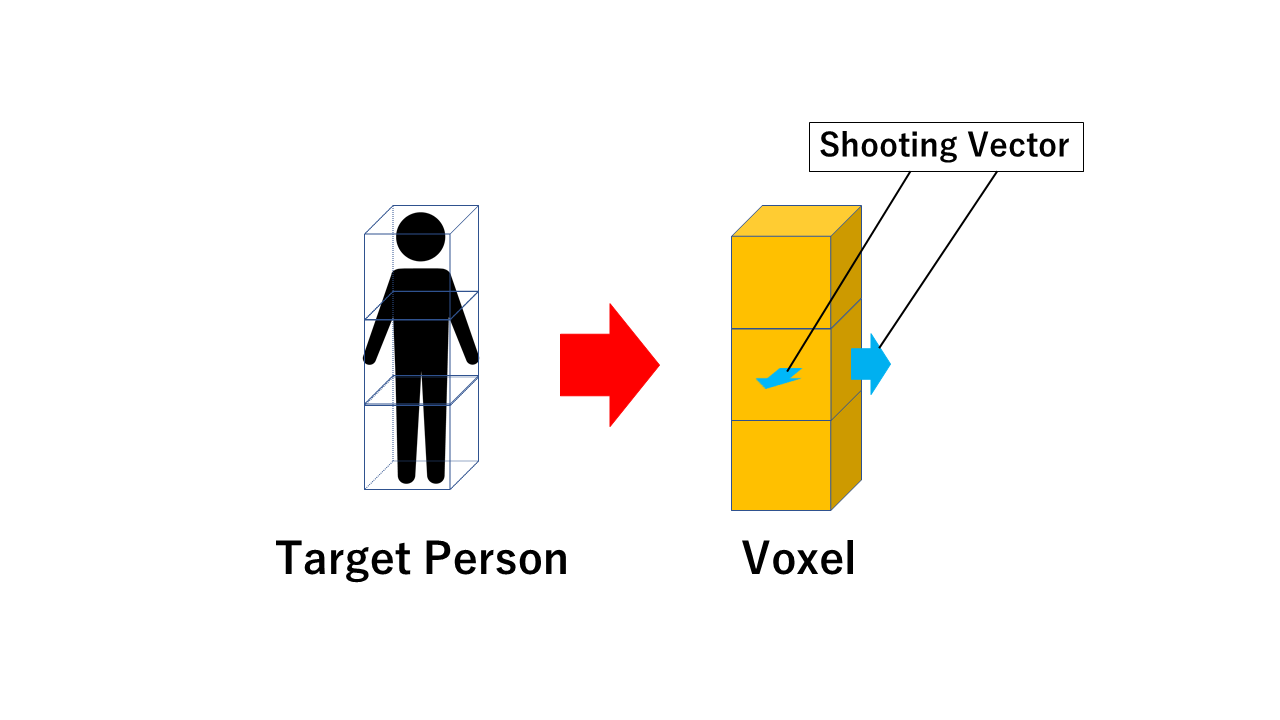
\includegraphics[width=\linewidth, clip]{./figure/chapter2/voxel.png}
    \caption{Model of Shooting Vector}
    \label{fig:voxel}
\end{figure}

\subsection{要求解像度}
この研究では,1[mm]を表すために必要な画素数[pixel/mm]で解像度を表現する.
あるカメラが撮影対象を撮影しているとき,カメラの水平(垂直)解像度を$R_{camera}$,
カメラの水平(垂直)画角を$\alpha$[rad],撮影対象を写している水平(垂直)画角を$\beta$とし,
セルの1辺の長さが$S$[mm]であるときの,撮影対象の解像度$R$[pixel/mm]は\cref{eq:pixel_mm}
で求められる.

\begin{equation}
    \label{eq:pixel_mm}
    \begin{aligned}
        \frac{\beta R_{camera}}{\alpha S}\mathrm{[pixel/mm]}
    \end{aligned}
\end{equation}

任意の要求解像度$n$[pixel/mm]が与えられたとき,要求解像度の満たすための条件は
\cref{eq:pixel_mm}より$n \le R$で表される.
この式より,要求解像度を満たすためには画角$\beta$に対して\cref{eq:angle_rule}を満足する必要がある.

\begin{equation}
\beta \le \frac{\alpha n S}{R_{camera}}\mathrm{[rad]}
\label{eq:angle_rule}
\end{equation}

以上より,ある撮影ベクトルについて要求解像度を満たす撮影領域は,
条件\cref{eq:angle_rule}を満たす水平画角$\beta_h$,垂直画角$\beta_v$の点の軌跡である.

\subsection{撮影領域の導出}
撮影領域の導出を平面について順番に導出していく.まず始めにx,y平面について考える.
撮影ベクトルが設定されたセルの中心を原点とするx,y座標系を考える.カメラの座標を($x$,$y$)[mm],撮影ベクトルとx軸のなす角を$\gamma$,セルの1辺の長さを2$\lambda$[mm]とすると水平画角$\beta_h$はのようになる.

\begin{equation}
\beta_{h}=\left|\arctan \left(\frac{y+\lambda \cos \gamma}{x-\lambda \sin \gamma}\right)-
               \arctan \left(\frac{y-\lambda \cos \gamma}{x+\lambda \sin \gamma}\right)\right|
\label{eq:beta_h_1}
\end{equation}

簡単のために$\gamma=0$のときを考えると,xy平面における水平画角$\beta_h$で捉えることのできる点の軌跡は
\cref{eq:beta_h_2}のようになる.

\begin{equation}
    \begin{aligned}
    \left(  x - \frac{\lambda}{\tan \beta_{h}}  \right) ^2 + y^2 & = \left( \frac{\lambda}{\tan \beta_{h}} \right) ^2 + \lambda^2
    \end{aligned}
\label{eq:beta_h_2}
\end{equation}

\section{脚先の高さの取り扱い}





\section{計画問題の定式化と解法}
\Cref{eq:state_input_model}より,$k$ステップ後の状態$\bm{q}^k$は初期状態$\bm{q}^0$と
入力列$\bm{U}_k = ( {\bm{u}^0}^T , \dots ,\, {\bm{u}^{k - 1}}^T )^T$を用いて
$\bm{q}^k = \bm{G}_k ( \bm{q}^0 ,\, \bm{U}_k )$と表すことができる.
目標状態$\bm{q}_{\goal}$へ$k$ステップで到達するとしたときの脚配置計画問題は,
\cref{eq:planning_problem_origin}の非線形代数方程式の解$\bm{U}_k$を求める逆運動学問題となる.
\begin{equation} \label{eq:planning_problem_origin}
    \bm{q}_{\goal} = \bm{G}_k \left( \bm{q}^0 ,\, \bm{U}_k \right)
\end{equation}
この問題\cref{eq:planning_problem_origin}を$\bm{U}_k$について解けば脚配置計画が求まる.

本論文では,目標追従を評価関数で表し,制約条件下での最適化問題として解くことを考える.
$\bm{U}_k$,$\bm{q}^0$を変数とする評価関数を$V = H ( \bm{q}^0 ,\, \bm{U}_k )$,
制約条件を$\bm{\omega} ( \bm{q}^0 ,\, \bm{U}_k ) \geq \bm{0}$として,
\cref{eq:nonlinear_minimize_problem}の最適化問題を定義する.
\begin{equation} \label{eq:nonlinear_minimize_problem}
    \begin{aligned}
        & \mathrm{minimize} && V = H \left( \bm{q}^0 ,\, \bm{U}_k \right) \\
        & \mathrm{subject~to} && \bm{\omega} \left( \bm{q}^0 ,\, \bm{U}_k \right) \geq \bm{0}
    \end{aligned}
\end{equation}

この\cref{eq:nonlinear_minimize_problem}の非線形計画問題を,反復法を用いて解くことを考える.
反復のある段階での入力列$\bm{U}_k$に微小変化$\bm{\Delta U}_k$を加えて$\bm{U}_k \gets \bm{U}_k + \bm{\Delta U}_k$として更新するとき,
更新前の評価値$V_{\now}$は,更新後の評価値$V_{\nxt}$と
変化量$\Delta V$を用いて$V_{\nxt} = V_{\now} + \Delta V$と表すことができる.
線形近似を用いて$V_{\nxt}$を$\bm{\Delta U}_k$に関する二次形式,制約条件を一次式に近似し,
更新量$\bm{\Delta U}_k$を求める問題を\cref{eq:quadratic_programming_problem_base}の
制約条件付きの二次計画問題に定式化する.
\begin{equation} \label{eq:quadratic_programming_problem_base}
    \begin{aligned}
        & \mathrm{minimize} && \Delta V = \frac{1}{2} \, \bm{\Delta U}_k^T \varPhi \, \bm{\Delta U}_k + \bm{\phi}^T \bm{\Delta U}_k \\
        & \mathrm{subject~to} && \varOmega \, \bm{\Delta U}_k + \bm{\omega} \geq \bm{0}
    \end{aligned}
\end{equation}
この問題\cref{eq:quadratic_programming_problem_base}を逐次解いて$\bm{U}_k$を更新していくことで,計画問題の解が得られる.

なお,以降では入力列更新前と後の変数をそれぞれ$(\mathrm{variable\_name})_{\now}$,$(\mathrm{variable\_name})_{\nxt}$の形で表すこととする.


\section{評価関数}
本論文では,目標状態到達を計画の指標とし,最適化する評価関数には目標追従二乗誤差を用いる.
\begin{equation} \label{eq:evaluation_function}
    V = \frac{1}{2} \, {\left\| \bm{\varepsilon} \right\|}^2 = \frac{1}{2} \, {\left\| \, \bm{q}_{\goal} - \bm{q}^k \right\|}^2_{K_p}
\end{equation}
$K_p$は重み行列である.
これを\cref{eq:nonlinear_minimize_problem}の問題の評価関数として設定する.
なお,目標追従以外の指標(\cite{yao_2010iros, yao_2011rs}における運動エネルギなど)も評価関数に加える事で最適化可能である.

問題\cref{eq:quadratic_programming_problem_base}へ適用するため,
$\bm{\Delta U}_k$によって更新された後の状態$\bm{q}^k_{\nxt}$を,
$\bm{q}^k_{\now}$の$\bm{U}_k$についてのヤコビ行列$J_k = \partial \bm{G}_k / \partial \bm{U_k}$を用いて線形近似する.
\begin{equation} \label{eq:q_next}
    \bm{q}^k_{\nxt} = \bm{q}^k_{\now} + J_k \, \bm{\Delta U}_k
\end{equation}
\Cref{eq:q_next}を用いて二次計画問題\cref{eq:quadratic_programming_problem_base}の評価関数を
\cref{eq:quadratic_programing_planning}で定義する.
\begin{equation}
\label{eq:quadratic_programing_planning}
    \begin{aligned}
        V_{\nxt} & = \frac{1}{2} \, {\left\| \bm{\varepsilon}_{\nxt} \right\|}^2_{K_p} + \frac{1}{2} \,{\left\| \bm{\Delta U}_k \right\|}^2_{K_u} + \frac{1}{2} \,{\left\| {\bm{\Delta U}_z}_k \right\|}^2_{K_{u_z}} \\
                  & = \frac{1}{2} \, {\left( \bm{\varepsilon}_{\now} - J_k \, \bm{\Delta U}_k \right)}^T K_p \left( \bm{\varepsilon}_{\now} - J_k \, \bm{\Delta U}_k \right) \\
                  % & \phantom{=} + \frac{1}{2} \, \bm{\Delta U}_k^T K_u \, \bm{\Delta U}_k + \frac{1}{2} \,{\left( {J_z}_k \, \bm{\Delta U}_k \right)}^T K_{u_z} \left( {J_z}_k \, \bm{\Delta U}_k \right) \\
                  & \phantom{=} + \frac{1}{2} \, \bm{\Delta U}_k^T K_u \, \bm{\Delta U}_k \\
                  & \phantom{=} + \frac{1}{2} \,{\left( {J_z}_k \, \bm{\Delta U}_k \right)}^T K_{u_z} \left( {J_z}_k \, \bm{\Delta U}_k \right) \\
                  & = \frac{1}{2} \, \bm{\Delta U}_k^T \varPhi \, \bm{\Delta U}_k + \bm{\phi}^T \bm{\Delta U}_k + \mathrm{const.} \\[5pt]
        \varPhi   & = J_k^T \, K_p J_k + K_u + {{J_z}_k^T} \, K_{u_z} {J_z}_k \\
        \bm{\phi} & = -J_k^T \, K_p \, \bm{\varepsilon}_{\now}
    \end{aligned}
\end{equation}
$K_p$,$K_u$,$K_{u_z}$は評価関数の各項を重み付ける対角行列である(対角成分の設定方法は\cref{sec:solve_qpp}に示す).
$\bm{\phi} \in R^{6k}$はベクトル,$\varPhi \in R^{6k \times 6k}$は実対称の正定値行列である.

\Cref{eq:quadratic_programing_planning}の式変形前の$V_{\nxt}$の定義において,
第一項は前述の目標追従二乗誤差の評価項,第二項は入力列の更新量$\bm{\Delta U}_k$最小化の評価項である.
第三項は,高さ変位を最小化するための項である.
脚配置モデルが状態として$z_l^i$,$z_r^i$を持つと仮定すると,\cref{eq:z_state_input_model}のように次ステップへ遷移すると考えられる.
\begin{equation} \label{eq:z_state_input_model}
    \begin{aligned}
        z_l^{i + 1} & = z_l^i + u_{zl}^i \\
        z_r^{i + 1} & = z_r^i + u_{zr}^i
    \end{aligned}
\end{equation}
高さに対する仮想的な入力$u_{zl}^i$,$u_{zr}^i$は\cref{eq:z_from_xy}を用いて$\bm{q}^i$,$\bm{q}^{i + 1}$,$z_{\field} ( x ,\, y )$から計算でき,
高さに対する仮想入力列${\bm{U}_z}_k = ( u_{zl}^0 ,\, u_{zr}^0 , \dots ,\, u_{zl}^{k - 1} ,\, u_{zr}^{k - 1} )^T$は$\bm{q}^0$,$\bm{U}_k$で表すことができる.
入力列更新時の${\bm{U}_z}_k$の変化${\bm{\Delta U}_z}_k$を最小化すれば,高さ方向の変位を最小化する計画が得られる.
なお,\cref{eq:quadratic_programing_planning}中の${J_z}_k$は,${\bm{U}_z}_k$の$\bm{U}_k$についての
ヤコビ行列${J_z}_k = \partial {\bm{U}_z}_k / \partial \bm{U}_k$である.


\section{制約条件}
\label{seq:constraints}
制約条件は,三次元上の脚配置を実現するために必要となる地形との接触についての制約と,
適用するロボットに合わせて定式化されるハードウェア上の制約からなる.

\subsection{地形との接触制約}
\label{subseq:field_contact_constraint}
平面上で定義されたモデルを用いて三次元の脚配置を実現するため,
地形との接触について制約を課す必要がある.
脚の垂直方向の移動が平面動作から独立していること,機構的に踏み出し時の高さには限界があることを踏まえ,
\cref{eq:z_from_xy}を用いて両脚間の高低差について制約を課す.
\begin{equation} \label{eq:z_field_const}
    \begin{gathered}
        -z_{\mathrm{max}} \leq z_l^{i + 1} - z_r^i \leq z_{\mathrm{max}} \\
        -z_{\mathrm{max}} \leq z_r^{i + 1} - z_l^{i + 1} \leq z_{\mathrm{max}}
    \end{gathered}
\end{equation}
$z_{\mathrm{max}}$は高低差の絶対値上限である.
この制約を課すと,歩行時の垂直方向の移動が上下限値内に収まるように歩幅を抑えた脚配置が求まることになり,
地形を考慮した脚配置計画が実現される.
地形形状に関しては,平面位置に対応する高さ$z_{\field} ( x ,\, y )$,
線形近似時に必要となる$x$,$y$方向それぞれの傾き$\partial z_{\field} / \partial x ,\, \partial z_{\field} / \partial y$が既知であればよい.
上限値$z_{\mathrm{max}}$は,定数としても関数としてもよい.
即ち,踏み出しの高さによって遊脚の水平方向の可動範囲が変化するような場合には,
$\bm{q}^i$,$\bm{u}^i$および$z_{\field}$を用いて表現される関数とするなど,
適用するロボットに合わせて定式化を行えばよい.

なお,現在は地形の傾斜に対する脚先の姿勢を考慮していない.
今後,脚裏形状や制御における許容範囲,地形形状情報から定式化できると考えている.



\subsection{遊脚の配置制約}
制約条件を定式化するために,\cref{fig:const_angle},\cref{fig:const_place}および\cref{fig:const_overlap}中に示している,次の三つのパラメータを定義する.
\begin{itemize}
    \item 支持脚と遊脚の相対距離$L^i$
    \item 支持脚の$y$軸から見た直線($L^i$)の傾き$\theta_1^i$
    \item 支持脚を中心としたときの両脚先間の相対角度$\theta_2^i$
\end{itemize}
$L^i$,$\theta_1^i$,$\theta_2^i$はそれぞれ,
右脚支持の場合に$L^i = l^i + u_{l1}^i$,$\theta_1^i = u_A^i - \theta^i + \theta_{fr}^i$,$\theta_2^i = \theta_{fl}^{i + 1} - \theta_{fr}^i$,
左脚支持の場合に$L^i = l^{i + 1}$,$\theta_1^i = \theta^{i + 1} - \theta_{fl}^{i + 1}$,$\theta_2^i = \theta_{fl}^{i + 1} - \theta_{fr}^{i + 1}$
となる.



まず,支持脚に対する遊脚の相対角度$\theta_2^i$に制約を課す.
これは\cref{eq:const_angle}で定式化される(\cref{fig:const_angle}参照).
\begin{equation}
    \label{eq:const_angle}
    {\theta_2}_{\mathrm{min}} \leq \theta_2^i \leq {\theta_2}_{\mathrm{max}}
\end{equation}
${\theta_2}_{\mathrm{max}}$,${\theta_2}_{\mathrm{min}}$は相対角度の上下限値である.


次に,支持脚に対する遊脚の可動範囲を\cref{fig:const_place}に示す領域内に制限する制約を課す.
支持脚に対する遊脚の相対位置座標$( x_{sw}^i ,\, y_{sw}^i ) = ( L^i \sin \theta_1^i ,\, L^i \cos \theta_1^i )$は,
$x_{sw}^i \geq 0$,$x_{sw}^i < 0$それぞれの範囲において,$( 0 ,\, Y_{\mathrm{min}} )$を中心とする楕円形の領域に制限されることとなる.
この楕円の径については,$x_{sw}^i \geq 0$,$x_{sw}^i < 0$それぞれの領域において,長軸は共通だが短軸は異なる.
\begin{equation}
\label{eq:const_place}
    \begin{gathered}
        y_{sw}^i \geq Y_{\mathrm{min}} \\ 
        \left( \frac{x_{sw}^i}{X} \right)^2 + \left( \frac{y_{sw}^i - Y_{\mathrm{min}}}{Y_{\mathrm{max}} - Y_{\mathrm{min}}} \right)^2 \leq 1.0 \\
        \left( X = 
        \begin{cases}
            X_{\mathrm{max}} & \left( x_{sw}^i \geq 0 \right) \\
            X_{\mathrm{min}} & \left( x_{sw}^i < 0 \right)
        \end{cases}
        \right)
    \end{gathered}
\end{equation}
$Y_{\mathrm{max}}$,$Y_{\mathrm{min}}$は$\Sigma_{sp}$の$y$軸上の両脚間隔の上限値及び下限値.
また,$X_{\mathrm{max}}$,$X_{\mathrm{min}}$は,脚間距離が最小のときの
前進・後進それぞれについての$\Sigma_{sp}$の$x$軸方向の歩幅上限値.

\subsection{脚先の干渉防止制約}
さらに,脚先が重なることを防ぐための制約を課す.
\cref{fig:const_overlap}に示している,支持脚座標系$\Sigma_{sp}$から見た遊脚の頂点$\bm{R}_A^i = (x_{R_A}^i ,\, y_{R_A}^i)$と$\bm{R}_B^i = (x_{R_B}^i ,\, y_{R_B}^i)$,
また遊脚座標系$\Sigma_{sw}$から見た左脚の頂点$\bm{L}_A^i = (x_{L_A}^i ,\, y_{L_A}^i)$と$\bm{L}_B^i = (x_{L_B}^i ,\, y_{L_B}^i)$は\cref{eq:sole_corner}で表される.
\begin{equation}
\label{eq:sole_corner}
    \begin{aligned}
        x_{R_A}^i & = L^i \sin \theta_1^i + O_{xf} \cos \theta_2^i + O_{yi} \sin \theta_2^i \\
        y_{R_A}^i & = L^i \cos \theta_1^i + O_{xf} \sin \theta_2^i - O_{yi} \cos \theta_2^i \\
        x_{R_B}^i & = L^i \sin \theta_1^i - O_{xb} \cos \theta_2^i + O_{yi} \sin \theta_2^i \\
        y_{R_B}^i & = L^i \cos \theta_1^i - O_{xb} \sin \theta_2^i - ^iO_{yi} \cos \theta_2^i \\
        x_{L_A}^i & = L^i \sin \left( - \theta_1^i - \theta_2^i \right) + O_{xf} \cos \theta_2^i + O_{yi} \sin \theta_2^i \\
        y_{L_A}^i & = L^i \cos \left( - \theta_1^i - \theta_2^i \right) + O_{xf} \sin \theta_2^i - O_{yi} \cos \theta_2^i \\
        x_{L_B}^i & = L^i \sin \left( - \theta_1^i - \theta_2^i \right) - O_{xb} \cos \theta_2^i + O_{yi} \sin \theta_2^i \\
        y_{L_B}^i & = L^i \cos \left( - \theta_1^i - \theta_2^i \right) - O_{xb} \sin \theta_2^i - O_{yi} \cos \theta_2^i 
    \end{aligned}
\end{equation}
%

%
提案するモデルにおける脚先形状は実際のロボットの脚先を包含できる最小の長方形としている.
$O_{yi}$$O_{yo}$はそれぞれ脚先中心から内側および外側の辺までの長さ,$O_{xf}$,$O_{xb}$はそれぞれ脚先中心から前端,後端までの長さである.
また,入力列の更新前後で制約式が不連続に変化するのを防ぐために,
\cref{fig:const_sole}に示すような左脚座標系から見た左脚内側,右脚座標系から見た右脚内側の形状を表現する関数$f_f ( x )$を導入する.
%
脚先座標系の$y$軸の正の方向に凸で,パラメータによって矩形に近づけられる関数が望ましく,
本論文では三つのパラメータ$a$,$b$,$c$をもつ$x$の$10$乗の関数とした.
\begin{equation} \label{eq:foot_shape}
    f_f ( x ) = a \, ( x - b )^{10} + c
\end{equation}
パラメータはLevenberg-Marquardt法による非線形最小二乗推定によりフィッティングを行った.
これを用いて,制約条件を\cref{eq:overlap_const}で表現する.
\begin{equation} \label{eq:overlap_const}
    \begin{aligned} 
        f_f \left( x_{R_A}^i \right) & \leq y_{R_A}^i &,&& f_f \left( x_{R_B}^i \right) & \leq y_{R_B}^i , \\ 
        f_f \left( x_{L_A}^i \right) & \leq y_{L_A}^i &,&& f_f \left( x_{L_B}^i \right) & \leq y_{L_B}^i
    \end{aligned}
\end{equation}

\subsection{二次計画問題への適用}
以上の制約条件$\omega_i(\bm{q}^0 ,\, \bm{U}_k) \geq 0 \ (i = 0 , \dots ,\, 20k - 1)$は,まとめて$\bm{\omega} ( \bm{q}^0 ,\, \bm{U}_k ) = ( \omega_0 , \dots ,\, \omega_{20 k - 1} )^T \geq \bm{0}\ ( \bm{\omega }\in R^{20k} )$と表される.
これを問題\cref{eq:quadratic_programming_problem_base}に適用するため,更新後の制約条件について線形近似を行う.
\begin{equation}\begin{aligned} 
    \bm{\omega}_{\nxt} = \bm{\omega}_{\now} + \varOmega \, \bm{\Delta U_k} \geq \bm{0}
\end{aligned}\end{equation}
$\varOmega \in R^{20k \times 6k}$は$\bm{\omega}_{\now}$の$\bm{U}_k$についてのヤコビ行列$\varOmega = \partial \bm{\omega}_{\now} / \partial \bm{U}_k$である.


\section{本章のまとめ}
本章では,三次元適応のための歩行モデルの拡張および追加の制約条件について説明した.
従来の水平方向の脚配置計画のためのモデルに,独立した垂直方向の動作を追加し,
脚配置遷移モデルの状態および入力についての次元の拡張を行うことなく,
事前に与えられた地形情報に基いて垂直方向の移動量を制限する制約を定式化し追加することで,
計算コスト増加を抑えつつ三次元地形への適応を可能にした.
次章では,本章で定義した計画問題の解法について,
全体のアルゴリズムおよび求解性能の安定化のためのいくつかの手法について述べる.


\end{document}
